\documentclass[letterpaper]{article} % DO NOT CHANGE THIS
\usepackage[submission]{aaai2027}  % DO NOT CHANGE THIS
\usepackage[hyphens]{url}  % DO NOT CHANGE THIS
\usepackage{graphicx} % DO NOT CHANGE THIS
\urlstyle{rm} % DO NOT CHANGE THIS
\def\UrlFont{\rm}  % DO NOT CHANGE THIS
\usepackage{natbib}  % DO NOT CHANGE THIS AND DO NOT ADD ANY OPTIONS TO IT
\usepackage{caption} % DO NOT CHANGE THIS AND DO NOT ADD ANY OPTIONS TO IT
\frenchspacing  % DO NOT CHANGE THIS
\usepackage{booktabs}
\usepackage{amsmath}
\usepackage{amssymb}
\usepackage{amsthm}

\pdfinfo{
/TemplateVersion (2027.1)
}

\setcounter{secnumdepth}{1}

\newtheorem{theorem}{Theorem}
\newtheorem{lemma}{Lemma}
\newtheorem{proposition}{Proposition}
\theoremstyle{remark}
\newtheorem*{remark}{Remark}

\newcommand{\Dstar}[1]{D^{\ast}_{#1}}
\newcommand{\Lp}{L_\varphi}
\newcommand{\lb}{\bar\lambda}
\newcommand{\R}{\mathbb{R}}

\title{How Far Can a Learned Market Simulator Miss a Liquidation Cascade?\\Error Bounds near Criticality}
\author{
    Anonymous Submission
}
\affiliations{
}

\begin{document}

\maketitle

\begin{abstract}
Generative world models are being proposed as simulators for financial stress tests: learn how agents and markets respond, then roll the model forward under shocks that have not happened. For credit, the outcome that matters most is the liquidation cascade, where forced sales move the price, which triggers more forced sales. We ask how an error in what such a model learns becomes an error in the cascade it predicts. Working with the liquidation map, the distribution of collateral by the price drop that would force its sale, we show that map error acts exactly like an error in the shock, and that the cascade turns shock error into size error through the slope $1/(1-\bar\lambda)$, where $\bar\lambda$ is the local branching ratio. The bound is sharp, it breaks by an order-one amount when a wall of positions sits within reach, and any model whose state is a finite set of aggregates has an error floor. Two quantities stay reliable near criticality: the shock that breaches a given price level, and tail risk under shifted shocks. A change to the liquidation threshold is an exact shock shift, so the rule-driven part of a governance change is no harder to predict than an ordinary cascade. On-chain lending, where every position is public, makes each prediction testable.
\end{abstract}

\section{Introduction}

Credit risk models are usually fit to historical outcomes, and they break when conditions shift, which is when they matter most. A world model, a learned simulator of how a system evolves given its state and the forces acting on it \citep{ha2018recurrent,hafner2025dreamerv3}, promises more: run the system forward under scenarios that never happened. Financial versions are starting to appear, from state representations of equity markets \citep{merchant2026financial} to language-model agents acting as borrowers in lending protocols \citep{li2026llmborrowers}, alongside hand-built market simulators \citep{byrd2019abides} and agent-based stress tests used by protocol risk teams \citep{kao2020compound}.

A stress test is only as good as its tail, and in credit the tail is the liquidation cascade. A price drop pushes leveraged positions under their liquidation threshold. Their collateral is sold, which pushes the price down further and liquidates more positions. Decentralized (on-chain) lending protocols run this loop in public code: every position, liquidation and parameter change is recorded \citep{qin2021liquidations}, and liquidators' sales move prices on decentralized exchanges \citep{lehar2022fragility}. That makes on-chain lending a clean testbed for any simulator that claims to predict cascades.

This paper asks a narrow question that any such simulator must answer: \emph{if the model's picture of the positions at risk is off by $\eta$, how far off is its cascade?} The answer has two halves. First, map error is shock error: a model with a wrong liquidation map predicts exactly what the true market would do under a shock shifted by at most $\Lp\eta$, with no amplification and no conditions (Lemma~\ref{lem:shock}). Second, the cascade reads that sideways error off its own curve, whose slope is $1/(1-\lambda)$ for local branching ratio $\lambda$. So size error grows without bound near criticality (Theorem~\ref{thm:stability}), as Figure~\ref{fig:error} shows.

\paragraph{Contributions.} We give
(i) a sharp stability bound for a learned model's cascade prediction, with an explicit interval on which it holds (Theorem~\ref{thm:stability}, Proposition~\ref{prop:sharp});
(ii) its failure mode, an order-one jump when a wall of positions sits within the bound's radius (Proposition~\ref{prop:wall}), and an error floor for every model whose state is a finite set of aggregates (Proposition~\ref{prop:aggregate});
(iii) two quantities that stay reliable near criticality, breach shocks and bracketed tail risk (Propositions~\ref{prop:breach} and~\ref{prop:tail});
(iv) an exact identity turning a liquidation-threshold change into a shock shift (Proposition~\ref{prop:threshold}), which links cascades to evaluating rule changes; and
(v) the two model constants these results need, derived from a liquidator selling on an exchange pool.
Every result is proved in the appendix and checked numerically on random liquidation books.

\paragraph{What is not new.} The $1/(1-\lambda)$ multiplier for shocks is classic \citep{brunnermeier2009liquidity}, with a matrix form for fire-sale spillovers \citep{greenwood2015vulnerable}. Fire-sale fixed points can jump \citep{cifuentes2005liquidity,cao2023pricemediated}, and threshold distributions, not aggregates, decide cascades \citep{granovetter1978threshold,onaga2022firesales}. Theorem~\ref{thm:stability} uses the textbook perturbation argument for contractions. What we did not find stated is the package for \emph{model} error: map error as shock error, the sharp slope and its failure radius, the aggregate floor, and the quantities that survive near criticality.

\paragraph{Related work.} Learned world models plan inside a model of the environment \citep{ha2018recurrent} and now span many control tasks \citep{hafner2025dreamerv3}; their error analysis rests on simulation lemmas \citep{kearns2002nearoptimal,ross2011reduction}, which bound error that compounds over time steps, not through a fixed point. Fire-sale and leverage models explain why cascades amplify and jump \citep{brunnermeier2009liquidity,cifuentes2005liquidity,cao2023pricemediated}, and on-chain studies document liquidations and their price impact \citep{qin2021liquidations,lehar2022fragility}. \citet{garciaseuma2026engine} measures a subcritical branching ratio for crypto derivatives and names the map of liquidation thresholds as the missing state variable. We connect these lines: given that map, how much can a learned simulator's error in it cost?

\section{Setup}

Work in log-price drops of one collateral asset, with the current price at drop $0$ and an exogenous shock $\delta$.
A \emph{liquidation map} $\mu$ is a finite measure on $\R$: $\mu(A)$ is the collateral force-sold by positions whose liquidation drop lies in $A$. Its forced-sale curve is $V_\mu(D)=\mu((-\infty,D])$. Price impact $\varphi:[0,\infty)\to[0,\infty)$ is nondecreasing and $\Lp$-Lipschitz with $\varphi(0)=0$. The cascade map and its outcome are
\begin{align}
T_\mu(D)&=\delta+\varphi\big(V_\mu(D)\big),\nonumber\\
\Dstar{\mu}(\delta)&=\min\{D\ge\delta : T_\mu(D)\le D\},
\label{eq:lfp}
\end{align}
the least fixed point, which exists by Tarski's theorem and is where round-by-round liquidation from $D_0=\delta$ stops. Where $V_\mu$ has density $f_\mu$, the slope of $T_\mu$ is the local branching ratio $\lambda=\varphi' f_\mu$: price impact times forced selling per unit drop, the quantity \citet{garciaseuma2026engine} measures for crypto derivatives. We write $\lb$ for a Lipschitz constant of $T_\mu$ on an interval. A world model predicts a map $\nu$, and its error is $\eta=\sup_D|V_\mu(D)-V_\nu(D)|$.

In a model with learned agents, $\nu$ is what the agent layer implies about who will be liquidated where; in an aggregate model it is whatever its state determines. The results below need nothing else from the model.

\section{Cascade Prediction Error}

\begin{lemma}[map error is shock error]\label{lem:shock}
For any maps $\mu,\nu$ and shock $\delta$, with $c=\Lp\eta$,
\[
\Dstar{\mu}(\delta-c)\ \le\ \Dstar{\nu}(\delta)\ \le\ \Dstar{\mu}(\delta+c).
\]
\end{lemma}

No slope condition is needed. The model's cascade curve sits within $\Lp\eta$ of the true one in the \emph{shock} direction. All size error comes from reading that sideways error off a steep curve.

\begin{theorem}[stability]\label{thm:stability}
Let $r=\Lp\eta/(1-\lb)$. If $T_\mu$ is $\lb$-Lipschitz on $I=[\delta,\ \Dstar{\mu}+r]$ with $\lb<1$, then $|\Dstar{\mu}-\Dstar{\nu}|\le r$.
\end{theorem}

The condition is on one map only, so $\nu$ can be the true book of discrete positions while $\mu$ is the model's smooth map. The proof caps $\Dstar{\nu}$ from above and rules out any fixed point of $T_\nu$ below $\Dstar{\mu}-r$, so the least fixed point cannot jump down. Liquidated volume carries the same factor: $|V_\mu(\Dstar{\mu})-V_\nu(\Dstar{\nu})|\le\eta/(1-\lb)$ when $\lb=\Lp\sup_I f_\mu$. Where the cascade curve is smooth, implicit differentiation gives $d\Dstar{\mu}/d\delta=1/(1-\lambda^\ast)$ exactly, so the factor is the true local sensitivity and not only an upper bound.

\begin{proposition}[sharpness]\label{prop:sharp}
For every $\lb\in(0,1)$, $\Lp>0$, $\delta>0$ and $\varepsilon>0$ there are maps with $T_\mu$ globally $\lb$-Lipschitz, $\eta=\varepsilon$ and $|\Dstar{\mu}-\Dstar{\nu}|=\Lp\varepsilon/(1-\lb)$.
\end{proposition}

\begin{proposition}[walls]\label{prop:wall}
Fix $\lambda_1<1$, $\Lp$, $\delta>0$ and a mass $m$. For every $\varepsilon>0$ there are maps with $\eta=\varepsilon$, $T_\mu$ $\lambda_1$-Lipschitz up to $\Dstar{\mu}+r/2$, a point mass $m$ at $\Dstar{\mu}+r/2$, and $\Dstar{\nu}-\Dstar{\mu}\ge\Lp m$.
\end{proposition}

A wall, a block of positions sharing one liquidation price such as loans opened at the maximum loan-to-value ratio, turns an arbitrarily small map error into an order-one cascade error. The jump itself is the known fire-sale discontinuity; what Proposition~\ref{prop:wall} adds is its reach. The radius $r$ grows without bound as $\lb\to1$, so near criticality a model must resolve every wall within a widening window.

\begin{proposition}[aggregates have a floor]\label{prop:aggregate}
Let $g_1,\dots,g_k$ be continuous with $1,g_1,\dots,g_k$ linearly independent on every tail $[B,\infty)$. For every wall mass $m$ there are maps $\mu,\nu$ with equal mass, $\int g_j\,d\mu=\int g_j\,d\nu$ for all $j$, and $|\Dstar{\mu}-\Dstar{\nu}|\ge\Lp m$.
\end{proposition}

Total collateral, total debt, and any number of moments of the liquidation drop are such aggregates. So a model whose state is a finite set of them errs by at least $\Lp m/2$ on one of two books it cannot tell apart, whatever it learns. This is Granovetter's point for threshold models, made explicit for liquidation maps, and it argues for state at the level of positions.

\paragraph{What stays reliable.} Near criticality a model cannot say how far a cascade runs. It can still say which shock breaks through a given level. For a level $w$, the \emph{breach shock} is $\delta^c_\mu(w)=\inf\{\delta:\Dstar{\mu}(\delta)\ge w\}$.

\begin{proposition}[breach shocks]\label{prop:breach}
For any maps and any level $w$, $|\delta^c_\mu(w)-\delta^c_\nu(w)|\le\Lp\eta$, with no slope condition.
\end{proposition}

\begin{proposition}[tails]\label{prop:tail}
Let $\delta$ be random and $R$ a $\beta$-quantile or $\mathrm{CVaR}_\beta$. Then $R(\Dstar{\mu}(\delta-c))\le R(\Dstar{\nu}(\delta))\le R(\Dstar{\mu}(\delta+c))$ with $c=\Lp\eta$. If Theorem~\ref{thm:stability} holds with radius at most $\bar r$ at every $\delta\ge\delta_{\mathrm{lo}}$, then $|R(\Dstar{\mu}(\delta))-R(\Dstar{\nu}(\delta))|\le\bar r$ for every $\beta>P(\delta<\delta_{\mathrm{lo}})$.
\end{proposition}

A stress test built on a learned model should therefore report breach shocks for known walls next to cascade sizes, and an estimate of $\lb$ next to both. Figure~\ref{fig:error} shows the contrast on random books: size error tracks $1/(1-\lb)$ and reaches it, while breach error stays below $\Lp\eta$ at every $\lb$.

\begin{figure}[t]
\centering
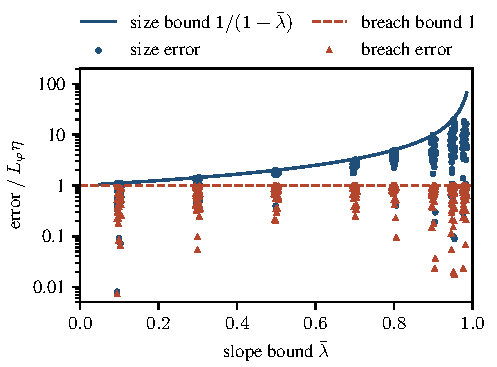
\includegraphics[width=\columnwidth]{figures/cascade_error.pdf}
\caption{Cascade size error and breach-shock error, in units of $\Lp\eta$, for 320 random pairs of nearby liquidation books (40 per slope bound $\lb$; exact least fixed points). Each pair misplaces a little selling near the current price. Size error stays under the bound of Theorem~\ref{thm:stability} and attains it; breach error stays under the bound of Proposition~\ref{prop:breach}. These are random books, not market data.}
\label{fig:error}
\end{figure}

\paragraph{Rule changes as shock shifts.} With one collateral asset, a position's liquidation drop is the log of its health factor, so changing the liquidation threshold from $\mathrm{LT}$ to $\mathrm{LT}'$ shifts every drop by $s=\log(\mathrm{LT}'/\mathrm{LT})$.

\begin{proposition}[threshold changes]\label{prop:threshold}
The shifted map $\mu_s$, with $V_{\mu_s}(D)=V_\mu(D-s)$, satisfies $\Dstar{\mu_s}(\delta)=s+\Dstar{\mu}(\delta-s)$ exactly.
\end{proposition}

The rule-driven part of a governance change is thus an ordinary cascade at a shifted shock, so its prediction error obeys Theorem~\ref{thm:stability}. To first order, lowering the threshold by $|s|$ deepens cascades by $|s|\lambda^\ast/(1-\lambda^\ast)$. A liquidation-bonus change scales the map instead, with the same $1/(1-\lambda^\ast)$ sensitivity. With $n$ collateral assets and an impact matrix $K$, the vector form holds with $r=(I-\Lambda)^{-1}K\eta$ for a nonnegative slope matrix $\Lambda$ of spectral radius below one. One asset can be subcritical alone while the system is critical through positions that hold several.

\section{Constants and Interventions}

\paragraph{Where $\Lp$ comes from.} A liquidator sells seized collateral on a constant-product pool with reserve $X$ and fee $f$, and an arbitrageur carries the move to the reference exchange, whose price feeds the protocol. If the exchange moves by $\psi$ per unit of flow over a reference reserve $X_0$, then to first order the transmitted impact is $\varphi(v)=\frac{k}{1+k}\varphi_{\mathrm{dex}}(v)$ with
\[
\Lp=\frac{\psi(1-f)}{X_0(1+k)},\qquad k=\frac{\psi(1-f)X}{(2-f)X_0},
\]
where $\varphi_{\mathrm{dex}}(v)=\log(X+v)+\log(X+(1-f)v)-2\log X$ is the pool's own impact. An arbitrage dead zone of width $\tau$ adds a fixed shock error $k\tau/(1+k)$ to the numerator of Theorem~\ref{thm:stability}. So $\Lp$ can be estimated from pool reserves rather than assumed, as the empirical work on liquidator price impact suggests \citep{lehar2022fragility}.

\paragraph{Smoothing.} Learning through liquidation eligibility needs a smooth surrogate of the indicator $\mathbb{1}[\log\mathrm{HF}<0]$. Replacing it with a logistic of width $h$ changes the forced-sale curve of any map with density at most $\rho$ by at most $\rho h\log 2$, which is attained, and when $\Lp\rho<1$ the smoothed cascade moves by at most $\Lp\rho h\log2/(1-\Lp\rho)$. A book of discrete positions has a floor of half its largest position for every $h$, which is why the model's smooth map, not the book, takes the role of $\mu$ in Theorem~\ref{thm:stability}.

\paragraph{When model error looks like behavior.} After a rule change, a model that holds agent behavior fixed predicts the rule-driven effect, and the residual mixes behavior change with model error. If agents act independently given the state, a multi-agent simulation lemma with a $\chi^2$ change of measure bounds the model error over a horizon $H$ by
\[
\mathrm{span}(Y)\sum_{t<H}\bar n_t\sqrt{1+\chi^2(d_t\,\|\,d^{\mathrm{obs}})}\ \varepsilon,
\]
where $d_t$ is the distribution of agent observations under the new rules, $d^{\mathrm{obs}}$ the training distribution, $\bar n_t$ the active agents and $\varepsilon$ the policies' in-distribution total-variation error, in $L^2$. This is standard technique \citep{kearns2002nearoptimal,ross2011reduction,metelli2018pois}, with the $\chi^2$ term estimable by a classifier density ratio \citep{bickel2009covariate}. It says when a residual can be read as behavior: only for rule changes whose overlap term stays small.

\section{Implications, Checks, and Limits}

\paragraph{For generative financial simulators.} The bounds are model-agnostic: they hold for a learned agent model, a sequence model of market states, or a language-model agent simulation, as long as it implies a liquidation map. Three practices follow. Report an estimate of $\lb$ and the radius $\hat r$ next to every predicted cascade, since the same map error costs $1/(1-\lb)$ times more near criticality. Report breach shocks for known walls, which keep their accuracy where cascade sizes lose it. And evaluate models whose state is aggregate on pairs of market states with matched aggregates, where Proposition~\ref{prop:aggregate} says they must fail. A model that is accurate on average can still be useless for stress testing if its error concentrates in the steep part of the cascade curve.

\paragraph{Numerical checks.} Each result is tested on random liquidation books built from point masses and piecewise-constant densities, with linear impact so that least fixed points are exact. The checks include a negative control: removing the $1/(1-\lb)$ factor from Theorem~\ref{thm:stability} must fail, and it does, so the tests are not vacuous. The constants of Section~4 are checked against simulated pools and arbitrage, and the smoothing bound and the simulation bound against random instances. All 40 checks pass: 13 for Section~3, 20 for the constants and smoothing, and 7 for the intervention bound. Code for every check and for Figure~\ref{fig:error} accompanies the submission.

\paragraph{Predictions for real data.} Each result names a measurement on chain data (Table~\ref{tab:predictions}). The inputs are estimable: $\hat\eta$ from per-address positions, $\hat L_\varphi$ from pool reserves, and $\hat\lambda$ from a smoothed map.

\begin{table}[t]
\centering
\footnotesize
\begin{tabular}{@{}p{0.13\columnwidth}p{0.19\columnwidth}p{0.56\columnwidth}@{}}
\toprule
Result & Error bound & Prediction to test on chain data \\
\midrule
Thm.~\ref{thm:stability} & $\Lp\eta/(1-\lb)$, sharp & Cascade error grows with $\hat\eta/(1-\hat\lambda)$ across historical shocks \\
Prop.~\ref{prop:wall} & $\ge\Lp m$ & Large misses concentrate where a wall sits within $\hat r$ of the predicted cascade \\
Prop.~\ref{prop:aggregate} & $\ge\Lp m/2$ & Aggregate models fail most on states with matched aggregates and different local mass \\
Props.~\ref{prop:breach}, \ref{prop:tail} & $\Lp\eta$ & Breach-shock error does not grow with $\hat\lambda$; tail risk is bracketed \\
Prop.~\ref{prop:threshold} & exact & Observed effect of a threshold change minus $s+\Dstar{}(\delta-s)-\Dstar{}(\delta)$ is behavior change \\
\bottomrule
\end{tabular}
\caption{Results, their bounds, and the measurement each predicts.}
\label{tab:predictions}
\end{table}

\paragraph{Limits.} The cascade is a one-shot fixed point. It ignores block timing, oracle delays and the order in which liquidations land. Impact is deterministic, borrowers do not top up inside the cascade, and the multi-asset form needs debt in stablecoins. The results bound error given $\eta$; they say nothing about how large a given model's $\eta$ is, which is an empirical question we leave to experiments on chain data.

\bibliography{references}

\appendix

\section{Proofs}

Throughout, $S_\mu(\delta)=\{D\ge\delta:T_\mu(D;\delta)\le D\}$, so that $\Dstar{\mu}(\delta)=\inf S_\mu(\delta)$ by Tarski's theorem. Equivalently, $\Dstar{\mu}(\delta)=\inf\{D\ge\delta:G_\mu(D)\ge\delta\}$ with $G_\mu(D)=D-\varphi(V_\mu(D))$. The set shrinks as $\delta$ grows, so $\Dstar{\mu}$ is nondecreasing in $\delta$. For every $D$, $|T_\mu(D)-T_\nu(D)|\le\Lp\eta$.

\paragraph{Lemma~\ref{lem:shock}.} Take $D\in S_\mu(\delta+c)$. Then $D\ge\delta$ and $\delta+\varphi(V_\nu(D))\le\delta+\varphi(V_\mu(D))+\Lp\eta=T_\mu(D;\delta+c)\le D$, so $S_\mu(\delta+c)\subseteq S_\nu(\delta)$ and taking infima gives the right inequality. Swapping $\mu$ and $\nu$ and replacing $\delta$ by $\delta-c$ gives the left one. \qed

\paragraph{Theorem~\ref{thm:stability}.} \emph{Upper bound.} Let $U=\Dstar{\mu}+r$. Then $T_\nu(U)\le T_\mu(U)+\Lp\eta\le T_\mu(\Dstar{\mu})+\lb r+\Lp\eta=\Dstar{\mu}+\lb r+(1-\lb)r=U$, so $U\in S_\nu(\delta)$ and $\Dstar{\nu}\le U$.
\emph{Lower bound.} Take $D\in[\delta,\Dstar{\mu}-r)$. The Lipschitz bound on $[D,\Dstar{\mu}]$ gives $T_\mu(D)\ge\Dstar{\mu}-\lb(\Dstar{\mu}-D)$, so $T_\nu(D)-D\ge T_\mu(D)-\Lp\eta-D\ge(1-\lb)(\Dstar{\mu}-D)-\Lp\eta>0$ because $\Dstar{\mu}-D>r$. No $D$ below $\Dstar{\mu}-r$ lies in $S_\nu(\delta)$, so $\Dstar{\nu}\ge\Dstar{\mu}-r$. \qed

The proof evaluates $T_\mu-T_\nu$ only on $I$, so $\eta$ may be replaced by $\sup_I|V_\mu-V_\nu|$. For volume, $\Dstar{\nu}\in I$, and splitting at $V_\mu(\Dstar{\nu})$ gives $|V_\mu(\Dstar{\mu})-V_\nu(\Dstar{\nu})|\le\rho r+\eta=\eta/(1-\lb)$ with $\rho=\sup_I f_\mu$ and $\lb=\Lp\rho$. For the local rate, if $\varphi$ is differentiable and $V_\mu$ has a density continuous near $\Dstar{\mu}$ with $\lambda^\ast<1$, the implicit function theorem applied to $D=\delta+\varphi(V_\mu(D))$ gives $d\Dstar{\mu}/d\delta=1/(1-\lambda^\ast)$, and the theorem keeps the least fixed point on that branch.

\paragraph{Proposition~\ref{prop:sharp}.} Take $\varphi(v)=\Lp v$, let $\mu$ have density $\lb/\Lp$ on $[0,K]$ with $K>(\delta+\Lp\varepsilon)/(1-\lb)$, and let $\nu=\mu+\varepsilon\mathbb{1}_{\{x_0\}}$ for some $x_0\in[0,\delta]$. On $[\delta,K]$, $T_\mu(D)=\delta+\lb D$ and $T_\nu(D)=\delta+\Lp\varepsilon+\lb D$, with least fixed points $\delta/(1-\lb)$ and $(\delta+\Lp\varepsilon)/(1-\lb)$, both below $K$. The gap is $\Lp\varepsilon/(1-\lb)$ and $\eta=\varepsilon$. \qed

\paragraph{Proposition~\ref{prop:wall}.} Take $\varphi(v)=\Lp v$, $s=\delta/(1-\lambda_1)$ and $g=\Lp\varepsilon/(2(1-\lambda_1))$. Let $\mu$ have density $\lambda_1/\Lp$ on $[0,s+g)$ plus a point mass $m$ at $s+g$, and let $\nu=\mu+\varepsilon\mathbb{1}_{\{0\}}$. Below the wall $T_\mu(D)=\delta+\lambda_1 D$, so $\Dstar{\mu}=s$. For $D<s+g$, $T_\nu(D)-D=(1-\lambda_1)(s+\Lp\varepsilon/(1-\lambda_1)-D)>0$, so $\nu$ has no fixed point below the wall. For $D\ge s+g$, $T_\nu$ is constant at $s+\lambda_1g+\Lp(\varepsilon+m)\ge s+g$, which is therefore $\Dstar{\nu}$. The gap is at least $\Lp m$, and $\eta=\varepsilon$. \qed

\paragraph{Proposition~\ref{prop:aggregate}.} Let $\beta$ be the wall book of Proposition~\ref{prop:wall} with $\varepsilon$ replaced by $t>0$, and pick $B$ beyond the reach of either cascade there, $B>s+\lambda_1 g+\Lp(t+m)$. Since $1,g_1,\dots,g_k$ are linearly independent on $[B,\infty)$, there are points $x_1<\dots<x_{k+1}$ in $[B,\infty)$ whose evaluation matrix $G$ is invertible. Let $x_0=0$, solve $Gw'=-(1,g_1(0),\dots,g_k(0))^\top$, and set $w=(1,w')$. The signed measure $\sigma=\sum_{i=0}^{k+1}w_i\mathbb{1}_{\{x_i\}}$ integrates $1$ and every $g_j$ to zero and has mass $1$ at drop $0$. Set $\mu=\beta+t\sigma^+$ and $\nu=\beta+t\sigma^-$. Both are nonnegative and agree on all $k+1$ aggregates. Below $B$, $\mu$ is $\beta$ plus mass $t$ at $0$ and $\nu$ is $\beta$, which is the pair of Proposition~\ref{prop:wall}; the far points lie beyond both cascades. So $|\Dstar{\mu}-\Dstar{\nu}|\ge\Lp m$. Polynomial moments together with the debt statistic $e^{-x}$ satisfy the independence condition, since they are analytic and independent on any interval. \qed

\paragraph{Proposition~\ref{prop:breach}.} By Lemma~\ref{lem:shock}, $\Dstar{\mu}(\delta)\ge w$ implies $\Dstar{\nu}(\delta+\Lp\eta)\ge w$, so $\delta^c_\nu(w)\le\delta^c_\mu(w)+\Lp\eta$. Swap the maps for the other side. \qed

\paragraph{Proposition~\ref{prop:tail}.} Quantiles and CVaR are monotone under almost-sure ordering, so the bracket follows from Lemma~\ref{lem:shock}. For the second part write $X=\Dstar{\mu}(\delta)$, $Y=\Dstar{\nu}(\delta)$, and replace $\delta$ by $\tilde\delta=\max(\delta,\delta_{\mathrm{lo}})$, giving $\tilde X,\tilde Y$ with $|\tilde X-\tilde Y|\le\bar r$ surely, so their quantiles differ by at most $\bar r$. Since $X<X(\delta_{\mathrm{lo}})$ forces $\delta<\delta_{\mathrm{lo}}$, $P(X<X(\delta_{\mathrm{lo}}))<\beta$, so $q_\beta(X)\ge X(\delta_{\mathrm{lo}})$ and $q_\beta(\tilde X)=q_\beta(X)$; likewise for $Y$. CVaR averages quantiles above $\beta$ and inherits the bound. \qed

\paragraph{Proposition~\ref{prop:threshold}.} Substitute $E=D-s$ in $S_{\mu_s}(\delta)$: the conditions $D\ge\delta$ and $\delta+\varphi(V_\mu(D-s))\le D$ become $E\ge\delta-s$ and $(\delta-s)+\varphi(V_\mu(E))\le E$. So $S_{\mu_s}(\delta)=s+S_\mu(\delta-s)$. Differentiating with the local rate gives $d\Dstar{}/ds=1-1/(1-\lambda^\ast)=-\lambda^\ast/(1-\lambda^\ast)$. For a bonus change from $b$ to $b'$, the map scales by $\kappa=(1+b')/(1+b)$, and implicit differentiation gives $d\Dstar{\kappa\mu}/d\kappa|_{\kappa=1}=\varphi'(V_\mu(\Dstar{\mu}))V_\mu(\Dstar{\mu})/(1-\lambda^\ast)$. \qed

\paragraph{Several assets.} With drops $D\in\R^n$, componentwise order, impact satisfying $|\varphi(v)-\varphi(w)|\le K|v-w|$ for a nonnegative matrix $K$, and $T_\mu(y)-T_\mu(x)\le\Lambda(y-x)$ for $x\le y$ in $[\delta,\Dstar{\mu}+r]$ with $\Lambda\ge0$ of spectral radius below one, let $r=(I-\Lambda)^{-1}K\eta$, so $r=\Lambda r+K\eta$. The upper bound repeats the scalar argument at $U=\Dstar{\mu}+r$. For the lower bound take $D$ with $T_\nu(D)\le D$, set $E=D\wedge\Dstar{\mu}$ and $g=\Dstar{\mu}-E\ge0$. Then $D\ge T_\nu(D)\ge T_\nu(E)\ge\Dstar{\mu}-\Lambda g-K\eta$, so $g_a\le(\Lambda g+K\eta)_a$ in every component with $g_a>0$, hence $(I-\Lambda)g\le K\eta$ and $g\le r$ because $(I-\Lambda)^{-1}\ge0$. \qed

\paragraph{Impact constant.} After selling $v$ on a pool with reserves $X,Y$ and fee $f$, the reserves are $X+v$ and $XY/(X+(1-f)v)$, which gives $\varphi_{\mathrm{dex}}$; it is concave with slope $(2-f)/X$ at $0$. Raising the pool's log price by $r$ takes $u=r(1-f)X/(2-f)+O(r^2)$ collateral, which moves the exchange by $\psi u/X_0=kr$. An arbitrage round closing a fraction $a$ of the gap $g_n$ leaves $g_{n+1}=g_n(1-a(1+k))$, which vanishes when $a(1+k)<2$, and the exchange moves by $kag_n$ per round, so the total is $\sum_n kag_0(1-a(1+k))^n=kg_0/(1+k)$ with $g_0=\varphi_{\mathrm{dex}}(v)$. Stopping once the gap is at most $\tau$ changes the total by at most $k\tau/(1+k)$, and Theorem~\ref{thm:stability}'s proof uses only the sup bound on $T_\mu-T_\nu$, so the extra term adds to its numerator. \qed

\paragraph{Smoothing.} Write $\sigma$ for the logistic function. The identity $|\mathbb{1}[x<0]-\sigma(-x/h)|=\sigma(-|x|/h)$ and $\int_0^\infty\sigma(-u/h)\,du=h\log2$ give, at each $D$, an error $A-B$ with $A,B\ge0$ each at most $\rho h\log2$, so $|V_\mu-V^h_\mu|\le\rho h\log2$; a uniform block attains it at its lower edge. The smoothed map has density at most $\rho$, so Theorem~\ref{thm:stability} with $\lb=\Lp\rho$ bounds the cascade shift. At an atom of mass $m$, $V_\mu$ jumps by $m$ while $V^h_\mu$ is continuous, so the error is at least $m/2$ on one side. \qed

\paragraph{Simulation bound.} Let $e(o)$ be the total-variation distance between the true and learned policies at observation $o$, and $\varepsilon=\|e\|_{L^2(d^{\mathrm{obs}})}$. Given the realized exogenous path, define hybrid trajectory laws that use the learned policy before step $k$ and the true one from step $k$ on. Consecutive hybrids differ only in the joint action law at step $k$, which under conditional independence is a product over agents, so their total-variation distance is at most $\mathbb{E}[\sum_i e(o_{i,k})]=\bar n_k\mathbb{E}_{d_k}[e]$. Summing over $k$ and multiplying by $\mathrm{span}(Y)$ bounds the outcome error. Finally, with $w=dd_t/dd^{\mathrm{obs}}$, Cauchy--Schwarz gives $\mathbb{E}_{d_t}[e]=\mathbb{E}_{d^{\mathrm{obs}}}[we]\le\sqrt{1+\chi^2(d_t\|d^{\mathrm{obs}})}\,\varepsilon$. \qed

\end{document}
